\documentclass[
  shownotes,
  xcolor={svgnames},
  hyperref={colorlinks,citecolor=DarkBlue,linkcolor=DarkRed,urlcolor=DarkBlue}
  , aspectratio=169]{beamer}
\usepackage{animate}
\usepackage{amsmath}
\usepackage{amsfonts}
\usepackage{amssymb}
\usepackage{pifont}
\usepackage{mathpazo}
%\usepackage{xcolor}
\usepackage{multimedia}
\usepackage{fancybox}
\usepackage[para]{threeparttable}
\usepackage{multirow}
\setcounter{MaxMatrixCols}{30}
\usepackage{subcaption}
\usepackage{graphicx}
\usepackage{lscape}
\usepackage[compatibility=false,font=small]{caption}
\usepackage{booktabs}
\usepackage{ragged2e}
\usepackage{chronosys}
\usepackage{appendixnumberbeamer}
\usepackage{animate}
\setbeamertemplate{caption}[numbered]
\usepackage{color}
%\usepackage{times}
\usepackage{tikz}
\usepackage{comment} %to comment
%% BibTeX settings
\usepackage{natbib}
\bibliographystyle{apalike}
\bibpunct{(}{)}{,}{a}{,}{,}
\setbeamertemplate{bibliography item}{[\theenumiv]}

% Defines columns for bespoke tables
\usepackage{array}
\newcolumntype{L}[1]{>{\raggedright\let\newline\\\arraybackslash\hspace{0pt}}m{#1}}
\newcolumntype{C}[1]{>{\centering\let\newline\\\arraybackslash\hspace{0pt}}m{#1}}
\newcolumntype{R}[1]{>{\raggedleft\let\newline\\\arraybackslash\hspace{0pt}}m{#1}}


\usepackage{xfrac}


\usepackage{multicol}
\setlength{\columnsep}{0.5cm}

% Theme and colors
\usetheme{Boadilla}

% I use steel blue and a custom color palette. This defines it.
\definecolor{andesred}{HTML}{af2433}

% Other options
\providecommand{\U}[1]{\protect\rule{.1in}{.1in}}
\usefonttheme{serif}
\setbeamertemplate{itemize items}[default]
\setbeamertemplate{enumerate items}[square]
\setbeamertemplate{section in toc}[circle]

\makeatletter

\definecolor{mybackground}{HTML}{82CAFA}
\definecolor{myforeground}{HTML}{0000A0}

\setbeamercolor{normal text}{fg=black,bg=white}
\setbeamercolor{alerted text}{fg=red}
\setbeamercolor{example text}{fg=black}

\setbeamercolor{background canvas}{fg=myforeground, bg=white}
\setbeamercolor{background}{fg=myforeground, bg=mybackground}

\setbeamercolor{palette primary}{fg=black, bg=gray!30!white}
\setbeamercolor{palette secondary}{fg=black, bg=gray!20!white}
\setbeamercolor{palette tertiary}{fg=white, bg=andesred}

\setbeamercolor{frametitle}{fg=andesred}
\setbeamercolor{title}{fg=andesred}
\setbeamercolor{block title}{fg=andesred}
\setbeamercolor{itemize item}{fg=andesred}
\setbeamercolor{itemize subitem}{fg=andesred}
\setbeamercolor{itemize subsubitem}{fg=andesred}
\setbeamercolor{enumerate item}{fg=andesred}
\setbeamercolor{item projected}{bg=gray!30!white,fg=andesred}
\setbeamercolor{enumerate subitem}{fg=andesred}
\setbeamercolor{section number projected}{bg=gray!30!white,fg=andesred}
\setbeamercolor{section in toc}{fg=andesred}
\setbeamercolor{caption name}{fg=andesred}
\setbeamercolor{button}{bg=gray!30!white,fg=andesred}


\usepackage{fancyvrb}
\newcommand{\VerbBar}{|}
\newcommand{\VERB}{\Verb[commandchars=\\\{\}]}
\DefineVerbatimEnvironment{Highlighting}{Verbatim}{commandchars=\\\{\}}
% Add ',fontsize=\small' for more characters per line
\usepackage{framed}
\definecolor{shadecolor}{RGB}{248,248,248}
\newenvironment{Shaded}{\begin{snugshade}}{\end{snugshade}}
\newcommand{\AlertTok}[1]{\textcolor[rgb]{0.94,0.16,0.16}{#1}}
\newcommand{\AnnotationTok}[1]{\textcolor[rgb]{0.56,0.35,0.01}{\textbf{\textit{#1}}}}
\newcommand{\AttributeTok}[1]{\textcolor[rgb]{0.77,0.63,0.00}{#1}}
\newcommand{\BaseNTok}[1]{\textcolor[rgb]{0.00,0.00,0.81}{#1}}
\newcommand{\BuiltInTok}[1]{#1}
\newcommand{\CharTok}[1]{\textcolor[rgb]{0.31,0.60,0.02}{#1}}
\newcommand{\CommentTok}[1]{\textcolor[rgb]{0.56,0.35,0.01}{\textit{#1}}}
\newcommand{\CommentVarTok}[1]{\textcolor[rgb]{0.56,0.35,0.01}{\textbf{\textit{#1}}}}
\newcommand{\ConstantTok}[1]{\textcolor[rgb]{0.00,0.00,0.00}{#1}}
\newcommand{\ControlFlowTok}[1]{\textcolor[rgb]{0.13,0.29,0.53}{\textbf{#1}}}
\newcommand{\DataTypeTok}[1]{\textcolor[rgb]{0.13,0.29,0.53}{#1}}
\newcommand{\DecValTok}[1]{\textcolor[rgb]{0.00,0.00,0.81}{#1}}
\newcommand{\DocumentationTok}[1]{\textcolor[rgb]{0.56,0.35,0.01}{\textbf{\textit{#1}}}}
\newcommand{\ErrorTok}[1]{\textcolor[rgb]{0.64,0.00,0.00}{\textbf{#1}}}
\newcommand{\ExtensionTok}[1]{#1}
\newcommand{\FloatTok}[1]{\textcolor[rgb]{0.00,0.00,0.81}{#1}}
\newcommand{\FunctionTok}[1]{\textcolor[rgb]{0.00,0.00,0.00}{#1}}
\newcommand{\ImportTok}[1]{#1}
\newcommand{\InformationTok}[1]{\textcolor[rgb]{0.56,0.35,0.01}{\textbf{\textit{#1}}}}
\newcommand{\KeywordTok}[1]{\textcolor[rgb]{0.13,0.29,0.53}{\textbf{#1}}}
\newcommand{\NormalTok}[1]{#1}
\newcommand{\OperatorTok}[1]{\textcolor[rgb]{0.81,0.36,0.00}{\textbf{#1}}}
\newcommand{\OtherTok}[1]{\textcolor[rgb]{0.56,0.35,0.01}{#1}}
\newcommand{\PreprocessorTok}[1]{\textcolor[rgb]{0.56,0.35,0.01}{\textit{#1}}}
\newcommand{\RegionMarkerTok}[1]{#1}
\newcommand{\SpecialCharTok}[1]{\textcolor[rgb]{0.00,0.00,0.00}{#1}}
\newcommand{\SpecialStringTok}[1]{\textcolor[rgb]{0.31,0.60,0.02}{#1}}
\newcommand{\StringTok}[1]{\textcolor[rgb]{0.31,0.60,0.02}{#1}}
\newcommand{\VariableTok}[1]{\textcolor[rgb]{0.00,0.00,0.00}{#1}}
\newcommand{\VerbatimStringTok}[1]{\textcolor[rgb]{0.31,0.60,0.02}{#1}}
\newcommand{\WarningTok}[1]{\textcolor[rgb]{0.56,0.35,0.01}{\textbf{\textit{#1}}}}
\usepackage{graphicx}
\makeatletter


% colors
\definecolor{airforceblue}{rgb}{0.36, 0.54, 0.66}
\newcommand{\theme}{\color{andesred}}
\newcommand{\bk}{\color{black}}
\newcommand{\rd}{\color{red}}
\newcommand{\fg}{\color{ForestGreen}}
\newcommand{\bl}{\color{blue}}
\newcommand{\gr}{\color{black!60}}
\newcommand{\sg}{\color{DarkSlateGray}}
\newcommand{\br}{\color{SaddleBrown}}
\newcommand{\nv}{\color{Navy}}


% common math markups
\newcommand{\bs}[1]{\boldsymbol{#1}}
\newcommand{\mc}[1]{\mathcal{#1}}
\newcommand{\mr}[1]{\mathrm{#1}}
\newcommand{\bm}[1]{\mathbf{#1}}
\newcommand{\ds}[1]{\mathds{#1}}
\newcommand{\indep}{\perp\!\!\!\perp}

% shorthand
\newcommand{\sk}{\vspace{.5cm}}
\newcommand{\R}[1]{{\tt \nv #1}}
\newcommand{\til}{{\footnotesize$\bs{\stackrel{\sim}{}}$}}
\DeclareSymbolFont{extraup}{U}{zavm}{m}{n}
\DeclareMathSymbol{\vardiamond}{\mathalpha}{extraup}{87}


\usepackage{tikz}
% Tikz settings optimized for causal graphs.
\usetikzlibrary{shapes,decorations,arrows,calc,arrows.meta,fit,positioning}
\tikzset{
    -Latex,auto,node distance =1 cm and 1 cm,semithick,
    state/.style ={ellipse, draw, minimum width = 0.7 cm},
    point/.style = {circle, draw, inner sep=0.04cm,fill,node contents={}},
    bidirected/.style={Latex-Latex,dashed},
    el/.style = {inner sep=2pt, align=left, sloped}
}


\makeatother






%%%%%%%%%%%%%%% BEGINS DOCUMENT %%%%%%%%%%%%%%%%%%

\begin{document}
 
\title[Lecture 25]{Lecture 25:   Text as Data}
\subtitle{Big Data and Machine Learning for Applied Economics \\ Econ 4676}
\date{\today}

\author[Sarmiento-Barbieri]{Ignacio Sarmiento-Barbieri}
\institute[Uniandes]{Universidad de los Andes}


\begin{frame}[noframenumbering]
\maketitle
\end{frame}

%%%%%%%%%%%%%%%%%%%%%%%%%%%%%%%%%%%




%----------------------------------------------------------------------% 

\begin{frame}
\frametitle{Agenda}

\tableofcontents

\end{frame}

%----------------------------------------------------------------------%
\section{Recap}
%----------------------------------------------------------------------%
\begin{frame}[fragile]
\frametitle{Super Learnets }


\begin{itemize}


\item Superlearning is a technique for prediction that involves combining many individual statistical algorithms  to create a new, single prediction algorithm that is expected to perform at least as well as any of the individual algorithms.
\medskip
\item The superlearner algorithm “decides” how to combine, or weight, the individual algorithms based upon how well each one minimizes a specified loss function
\medskip
\item The motivation for this type of “ensembling” is that a mix of multiple algorithms may be more optimal for a given data set than any single algorithm. 
\medskip
\item For example, a tree based model averaged with a linear model (e.g. random forests and LASSO) could smooth some of the model’s edges to improve predictive performance.
\end{itemize}

\end{frame}

%----------------------------------------------------------------------%
\begin{frame}[fragile]
\frametitle{Superlearnes: Summary}



  \begin{figure}[H] \centering
            \captionsetup{justification=centering}
              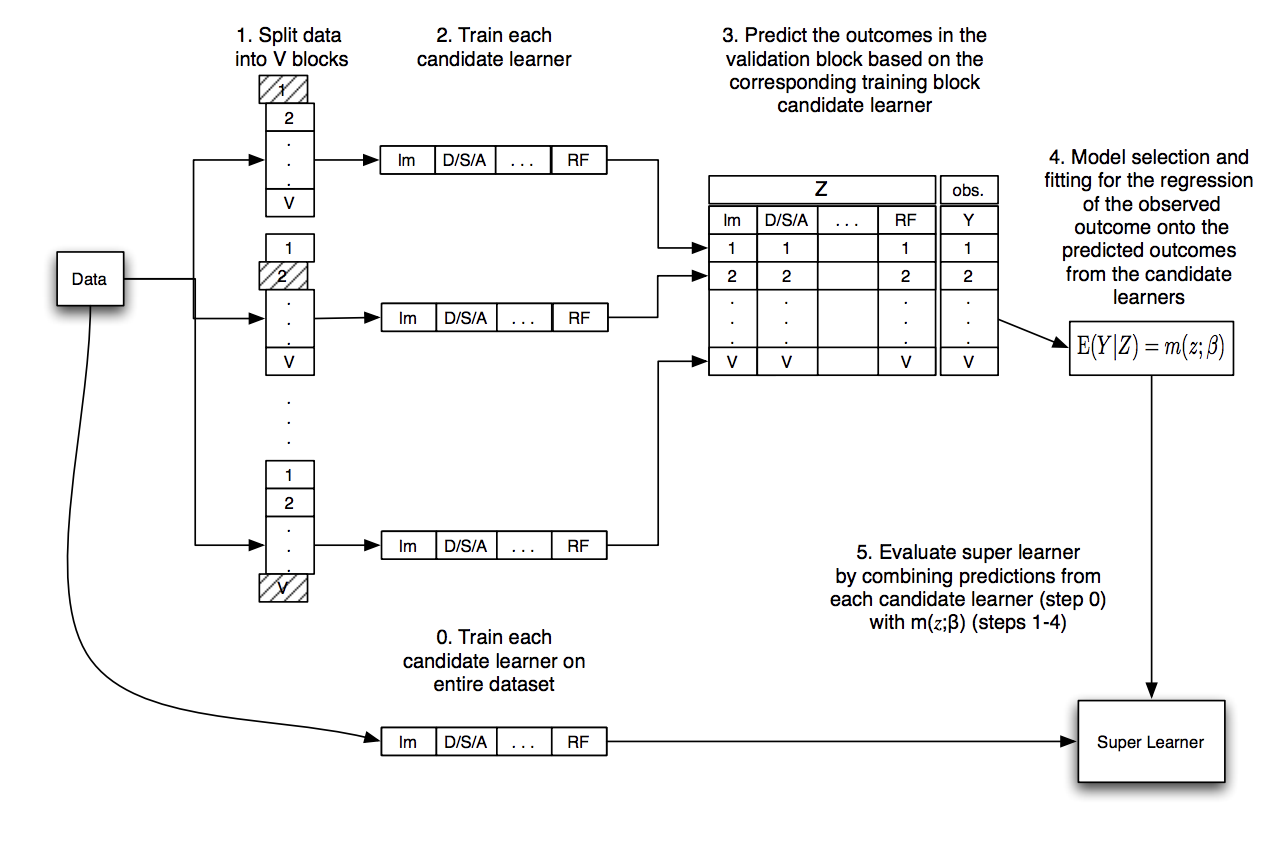
\includegraphics[scale=0.5]{../Lecture24/figures/sl_diagram.png}
              \\
              \tiny
              Source: Polley, Eric. Learning: Causal Inference for Observational and Experimental Data
 \end{figure}

\end{frame}
%----------------------------------------------------------------------%
\section{Text as Data}
%----------------------------------------------------------------------%
\begin{frame}[fragile]
\frametitle{}


\centering
{\huge \textcolor{andesred}{Text as Data}}


\end{frame}
%----------------------------------------------------------------------%
\begin{frame}[fragile]
\frametitle{Text as Data: The Big Picture}

\begin{itemize}


\item {\bf \theme Text is a vast source of data for research, business,etc }
\medskip
\item It comes connected to interesting ``author'' variables 
\medskip
  \begin{itemize}
  \item What you buy, what you watch, your reviews
  \medskip
  \item Group membership, who you represent, who you email
  \medskip
  \item Market behavior, macro trends, the weather
  \end{itemize}

 

\end{itemize}

\end{frame}
%----------------------------------------------------------------------%
\begin{frame}[fragile]
\frametitle{Text as Data: Motivation}


  \begin{figure}[H] \centering
            \captionsetup{justification=centering}
              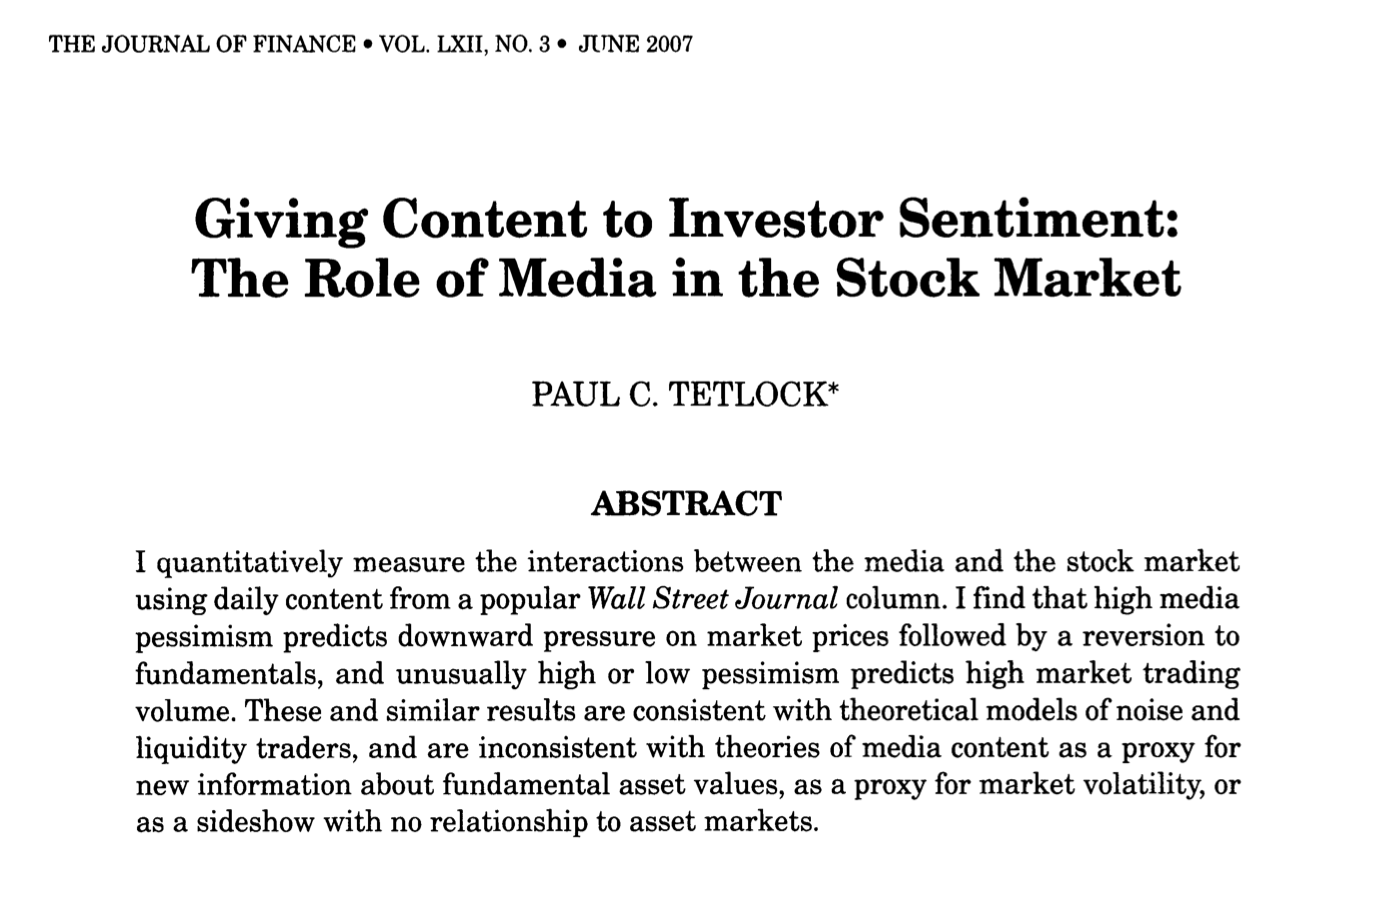
\includegraphics[scale=0.5]{figures/Tetlock.png}
              
 \end{figure}

\end{frame}

%----------------------------------------------------------------------%
\begin{frame}[fragile]
\frametitle{Text as Data: Motivation}


  \begin{figure}[H] \centering
            \captionsetup{justification=centering}
              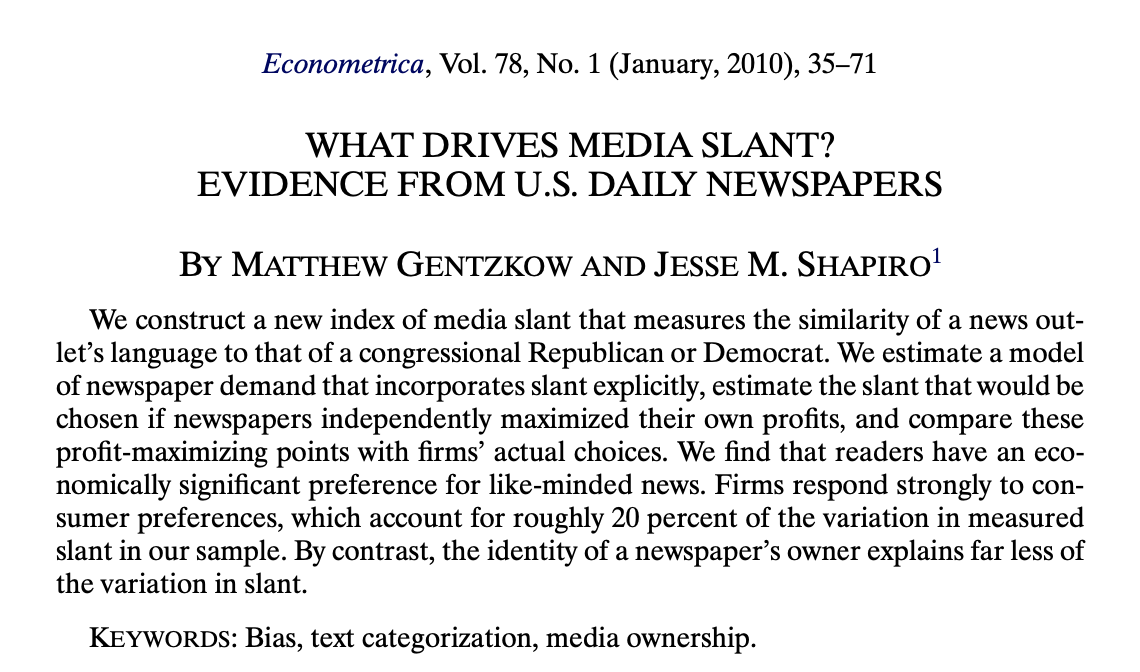
\includegraphics[scale=0.6]{figures/gentzgow_shapiro}
              
 \end{figure}

\end{frame}
%----------------------------------------------------------------------%
\begin{frame}[fragile]
\frametitle{Text as Data: Motivation}
\framesubtitle{Gentzkow and Shapiro: What drives media slant?  Evidence from U.S. daily newspapers ({\it Econometrica}, 2010)}

\begin{itemize}
\item Build an economic model for newspaper demand that incorporates political partisanship (\rd Republican \bk vs \bl Democrat\bk)

\medskip
 
\begin{itemize}
\item What would be independent profit-maximizing ``slant''?
\medskip
\item Compare this to slant estimated from newspaper text.
\end{itemize}
\medskip

\item Use data from Congress to isolate the phrases
\medskip
\item Compare phrase frequencies in the newspaper with phrase frequencies in the 2005 Congressional Record to identify whether the newspaper’s language is more similar to that of a congressional Republican or a congressional Democrat

\end{itemize}
\end{frame}

\begin{frame}[fragile]
\frametitle{Text as Data: Motivation}

\begin{itemize} 
  \item Jerry Moran, R-KS, says ``death tax'' relatively often and his district (Kansas 1st) voted 73\% for George W. Bush in 2004.

  \item William Jefferson, D-LA, says ``estate tax'' relatively often and his district voted 24\% for George W. Bush in 2004.

\medskip

$\bm{\Rightarrow}$ ``death tax'' is republican



\begin{align}
Ideology = f(\bm{X_\text{text}}) + u
\end{align}

where 
\begin{align}
ideology \approx g(Y_{Bush})
\end{align}

\item Gentzkow and Shapiro apply this logic to build an index of slant that sums across a speaker’s term usage weighted by the direction of slant for each term. 

\end{itemize}


\end{frame}


%----------------------------------------------------------------------%
\subsection{Turn Text into Data: Tokenization}
%----------------------------------------------------------------------%
\begin{frame}[fragile]
\frametitle{Turn Text into Data: Tokenization}


\begin{itemize}


\item Raw text—the language that humans read—is an incredibly rich object. 
\medskip
\item It is much more than a sum of words.
\medskip
 \item Meaning is built from ordered sequences of words that refer to each other, often separated across sentences or paragraphs. 
 \medskip
 \item However, the vast majority of text analyses will ignore this complexity and rely solely on counts for language tokens: words, phrases, or other basic elements. 
 \medskip
 \item Fortunately, a huge amount of information is contained in these simple counts. 
 \medskip
 \item The lesson of the past 30 years has been that, for prediction and classification with text, it is difficult to make effective use of any statistics other than simple word counts. 
 
\end{itemize}
\end{frame}
%----------------------------------------------------------------------%
\begin{frame}[fragile]
\frametitle{Turn Text into Data: Tokenization}
\begin{itemize}


\item A passage in `{\it As You Like It}' from Shakepeare:

\medskip

\begin{quote}
~~~ {\sg All the world's a stage,\\
~~~ and all the men and women merely players:\\
~~~ they have their exits and their entrances;\\
~~~ and one man in his time plays many parts...}
\end{quote}


\medskip
{\footnotesize
\item What the econometrian sees:

\medskip
\vspace{-.4cm}{\sg
\begin{verbatim}
   world stage men women play exit entrance time 
       1     1   2     1    2    1        1    1 
\end{verbatim}}
}
\medskip
\item This is the {\nv Bag-of-Words} representation of text.
\end{itemize}
\end{frame}



%----------------------------------------------------------------------%
\begin{frame}[fragile]
\frametitle{Turn Text into Data: Tokenization}
\begin{itemize}
\item This is the {\nv Bag-of-Words} representation of text.
\medskip
\item It treats documents as if they were constructed by randomly drawing words with-replacement from a bucket containing the fixed vocabulary. 
\medskip
\item By summarizing a document in terms of word counts, we are throwing away all information relevant to any more complex processes of document construction. 
\medskip
\item The advantage of this approach is its simplicity: you can characterize relationships between language and outside variables (e.g., authorship or sentiment) by building a model for word probabilities.

\end{itemize}
\end{frame}
%----------------------------------------------------------------------%
\begin{frame}[fragile]
\frametitle{Turn Text into Data: Tokenization}
\framesubtitle{Possible tokenization steps} 

\begin{itemize}
\item There are many possible algorithms for going from raw text to a summary token-count vector x.



\begin{quote}
~~~ {\sg All the world's a stage,\\
~~~ and all the men and women merely players:\\
~~~ they have their exits and their entrances;\\
~~~ and one man in his time plays many parts...}
\end{quote}


\item  A possible sequence is:
\begin{itemize}
\item Convert to lowercase, drop numbers, punctuation, etc ...\\
{\gr Always application specific: e.g., don't drop {\tt :-)} from tweets.}
\medskip

\item  Remove a list of {\nv stop words} containing  irrelevant tokens.\\
{\footnotesize
{\gr ~~~~~If, and, but, who, what, the, they, their, a, or, ...}

{\nv Be careful: one person's stopword is another's key term.}
}
\end{itemize}

\medskip
{\footnotesize
\item What the econometrian sees:

\medskip
\vspace{-.4cm}{\sg
\begin{verbatim}
   world stage men women play exit entrance time 
       1     1   2     1    2    1        1    1 
\end{verbatim}}
}


\end{itemize}

\end{frame}
%----------------------------------------------------------------------%
\begin{frame}[fragile]
\frametitle{Turn Text into Data: Tokenization}
\framesubtitle{Possible tokenization steps} 

\begin{quote}
~~~ {\sg All the world's a stage,\\
~~~ and all the men and women merely players:\\
~~~ they have their exits and their entrances;\\
~~~ and one man in his time plays many parts...}
\end{quote}


\begin{itemize}
\item Next
\begin{itemize}
\item Stemming:  `{\nv play}' $\leftarrow$   play,  players, ... 

{\gr A stemmer cuts words to their root with a mix of rules and estimation.`Porter' is standard for English. }
\end{itemize}
\medskip
{\footnotesize
\item What the econometrian sees:

\medskip
\vspace{-.4cm}{\sg
\begin{verbatim}
   world stage men women play exit entrance time 
       1     1   2     1    2    1        1    1 
\end{verbatim}}
}

\footnotesize
\item Also, remove words that are super rare {\gr (in say $<\frac{1}{2}$\%, or $<15\%$ of docs; this is application specific)}.
 For example, if {\nv Colombian} occurs only once, it's useless for comparing documents.




\end{itemize}

\end{frame}


%----------------------------------------------------------------------%
\begin{frame}[fragile]
\frametitle{The $n$-gram language model}

\begin{itemize}

\item One common strategy is to count n-grams, or combinations of n words, rather than single “unigrams”

\medskip

\item An {\theme $n$-gram tokenization} counts length-$n$ sequences of words.\\
{\sg A unigram is a word, bigrams are transitions between words.}\\
{\gr e.g., {\tt world.stage}, {\tt stage.men}, {\tt men.women}, {\tt women.play}, ...}

\medskip

\item This can give you rich language data, but be careful: $n$-gram token vocabularies are very high dimensional ($p^n$)
\medskip
\item  More generally, you may have domain specific `clauses' that you wish to tokenize.
\medskip
\item  There is always a trade-off between complexity and generality. 


\end{itemize}


\end{frame}

%----------------------------------------------------------------------%
\begin{frame}[fragile]
\frametitle{Turn Text into Data: Tokenization}

\begin{itemize}
  \item {\theme Often best to just count words.}
  \medskip
  \item For example, occurrences by party for some partisan terms

  \vskip .25cm
  \begin{table}[H]
  \centering
  
  \begin{tabular}{|c|c|c|c|c|c|c}
  Congress & State & Party & America & Death Tax & Estate Tax & $\cdots$
  \\ \hline
  \multirow{2}{*}{63} & \multirow{2}{*}{\sf NM} & {\sf dem}  & 108 &
    30 & 140 & \\ &
  & {\sf gop}  & 100 &
    220 & 12  &
  \end{tabular}
\end{table}

\end{itemize}


\end{frame}

%----------------------------------------------------------------------%
\begin{frame}[fragile]
\frametitle{Turn Text into Data: DTM}

\begin{itemize}
\item Once we have this clean text, we can convert from words to counts of words and create a document-term-matrix (DTM)
\medskip
\item $X$ that has a row for each document and a column for each word. 
\medskip
\item Element $x_{ij}$ is the count for word j in document i.
\medskip
\item This is highly sparse (sometimes we remove terms that have zero counts more than 75\% of the time)
\end{itemize}
\end{frame}
%----------------------------------------------------------------------%
\subsection{Text Regression}
%----------------------------------------------------------------------%
\begin{frame}
\frametitle{Text Regression}

\begin{itemize}
\item Once you have text in a numeric format, it will give us a powerful framework for text analysis.
\item When we combine with all the tools we learned so far



\medskip
\begin{align}
y= f(word\,counts) + u
\end{align}
 
\item where you can use ols, lasso, etc.

\end{itemize}
\end{frame}



%----------------------------------------------------------------------%
\begin{frame}[fragile]
\frametitle{Text Regression: Example (Gentzkow and Shapiro)}
\begin{scriptsize}



\begin{Shaded}
\begin{Highlighting}[]
\CommentTok{\#load packages}
\KeywordTok{library}\NormalTok{(textir) }
\CommentTok{\#load data}
\KeywordTok{data}\NormalTok{(congress109)}
\NormalTok{congress109Counts[}\KeywordTok{c}\NormalTok{(}\StringTok{"Barack Obama"}\NormalTok{,}\StringTok{"John Boehner"}\NormalTok{),}\DecValTok{995}\OperatorTok{:}\DecValTok{998}\NormalTok{]}
\end{Highlighting}
\end{Shaded}

\end{scriptsize}
\begin{tiny}


\begin{verbatim}
## 2 x 4 sparse Matrix of class "dgCMatrix"
##              stem.cel natural.ga hurricane.katrina trade.agreement
## Barack Obama        .          1                20               7
## John Boehner        .          .                14               .
\end{verbatim}

\end{tiny}
\begin{scriptsize}


\begin{Shaded}
\begin{Highlighting}[]
\NormalTok{congress109Ideology[}\DecValTok{1}\OperatorTok{:}\DecValTok{4}\NormalTok{,}\DecValTok{1}\OperatorTok{:}\DecValTok{5}\NormalTok{]}
\end{Highlighting}
\end{Shaded}
\end{scriptsize}
\begin{tiny}


\begin{verbatim}
##                            name party state chamber  repshare
## Chris Cannon       Chris Cannon     R    UT       H 0.7900621
## Michael Conaway Michael Conaway     R    TX       H 0.7836028
## Spencer Bachus   Spencer Bachus     R    AL       H 0.7812933
## Mac Thornberry   Mac Thornberry     R    TX       H 0.7776520
\end{verbatim}
\end{tiny}
\end{frame}

%----------------------------------------------------------------------%
\begin{frame}[fragile]
\frametitle{Text Regression}

\begin{itemize}
  \item We can use {\tt LASSO}
\end{itemize}
\begin{scriptsize}

\begin{Shaded}
\begin{Highlighting}[]
\NormalTok{f \textless{}{-}}\StringTok{ }\NormalTok{congress109Counts}
\NormalTok{y \textless{}{-}}\StringTok{ }\NormalTok{congress109Ideology}\OperatorTok{$}\NormalTok{repshare}
\CommentTok{\# lasso }
\NormalTok{lassoslant \textless{}{-}}\StringTok{ }\KeywordTok{cv.gamlr}\NormalTok{(congress109Counts}\OperatorTok{\textgreater{}}\DecValTok{0}\NormalTok{, y)}
\NormalTok{B \textless{}{-}}\StringTok{ }\KeywordTok{coef}\NormalTok{(lassoslant}\OperatorTok{$}\NormalTok{gamlr)[}\OperatorTok{{-}}\DecValTok{1}\NormalTok{,]}
\KeywordTok{head}\NormalTok{(}\KeywordTok{sort}\NormalTok{(}\KeywordTok{round}\NormalTok{(B[B}\OperatorTok{!=}\DecValTok{0}\NormalTok{],}\DecValTok{4}\NormalTok{)),}\DecValTok{10}\NormalTok{)}
\end{Highlighting}
\end{Shaded}

\end{scriptsize}
\begin{tiny}


\begin{verbatim}
##    congressional.black.caucu                 family.value 
##                      -0.0839                      -0.0443 
##        issue.facing.american           voter.registration 
##                      -0.0324                      -0.0298 
##      minority.owned.business            strong.opposition 
##                      -0.0284                      -0.0264 
##                  civil.right        universal.health.care 
##                      -0.0259                      -0.0254 
## congressional.hispanic.caucu          ohio.electoral.vote 
##                      -0.0187                      -0.0183
\end{verbatim}
\end{tiny}

\end{frame}
%----------------------------------------------------------------------%
\begin{frame}[fragile]
\frametitle{Text Regression}

\begin{scriptsize}

\begin{Shaded}
\begin{Highlighting}[]
\KeywordTok{tail}\NormalTok{(}\KeywordTok{sort}\NormalTok{(}\KeywordTok{round}\NormalTok{(B[B}\OperatorTok{!=}\DecValTok{0}\NormalTok{],}\DecValTok{4}\NormalTok{)),}\DecValTok{10}\NormalTok{)}
\end{Highlighting}
\end{Shaded}

\end{scriptsize}
\begin{tiny}

\begin{verbatim}
##         illegal.alien        percent.growth   illegal.immigration 
##                0.0079                0.0083                0.0087 
##            global.war          look.forward            war.terror 
##                0.0098                0.0099                0.0114 
##      private.property        action.lawsuit          human.embryo 
##                0.0133                0.0142                0.0226 
## million.illegal.alien 
##                0.0328
\end{verbatim}


\end{tiny}

\end{frame}
%----------------------------------------------------------------------%
\section{Factor Models}
%----------------------------------------------------------------------%
\begin{frame}
\frametitle{Factor Models}

\begin{itemize}
\item Text is super high dimensional
\medskip
\item There is often abundant {\it unlabeled} text
\medskip
\item Some times unsupervized factor model is a popular and useful strategy with text data
\medskip
\item You can first fit a factor model to a giant corpus and use these factors for supervised learning on a subset of labeled documents.
\medskip
\item The unsupervised dimension reduction facilitates the supervised learning
\end{itemize}
\end{frame}
%----------------------------------------------------------------------%
\begin{frame}
\frametitle{Factor Models}

\begin{itemize}


\item One way to think about almost everything we do is as dimension reduction.
\medskip
 \item We are trying to learn from high-dimensional x some low-dimensional summaries that contain the information necessary to make good decisions. 
 \medskip
 \item Dimension reduction can be supervised or unsupervised.
  \medskip
 \item In supervised learning, an outside  “response” variable y dictates the direction of dimension reduction.
  \medskip
  \begin{itemize}
   \item  In regression, a high-dimensional $X$ is projected through coefficients $\beta$ to create the low-dimensional (univariate) summary $\hat y$. 
  \end{itemize}


\end{itemize}
\end{frame}
%----------------------------------------------------------------------%
\begin{frame}
\frametitle{Factor Models}

\begin{itemize}

 \item In contrast, for unsupervised learning there is no response or outcome. 
 \medskip
 \item We have a high-dimensional $X$, and you try to model it as having been generated from a small number of components. 
 \medskip
 \item We are attempting to simplify $X$ for its own sake. 
 \medskip
 \item Why? For example, you might want to predict the sentiment of people from the words in their tweets; you will have a massive bank of all tweets (many $X$ observations) but for only a small percentage will you know whether they are expressing positive or negative sentiment (e.g., by hand-labeling the tweets using human readers). 
 \medskip
 \item An unsupervised analysis will use all of the tweets to break the content into topics, and then you can easily sort these topics by sentiment on the subset of labeled tweets. 

\end{itemize}
\end{frame}
%----------------------------------------------------------------------%
\begin{frame}
\frametitle{Factor Models}

\begin{itemize}

 \item We’ll explore different methods of factorization—tools that break the expectation for each $X$ into the sum of a small number of factors.
\medskip
\item Let's then model the task
\medskip
\pause
\item Given a matrix of high-dimensional data $X_{n\times p}$, you’d like to reduce this to a function of a few “important” factors. 

\item We do this by building a linear model for x as a function of these unknown factors and then estimating both factors and model at the same time.


\end{itemize}
\end{frame}
%----------------------------------------------------------------------%
\begin{frame}
\frametitle{Factor Models}

\begin{itemize}
\item A factor model looks like 

\begin{align}
x_{ij}=  \phi_{i1} f_{j1} + \dots + \phi_{ik} f_{jk} \,\, j=1,\dots,p
\end{align}

\item where 
  \begin{itemize}
   \item $x_{ij}$ are the inputs of the regressions (independent vars)
   \medskip
   \item The $f_{ik}$ values are attached to each observation; they are like the $x_{ij}$ inputs in regression, except that they are now unknown latent factors that need to be estimated.
  \medskip
   \item $\phi_{jk}$ coefficients are called loadings or rotations—these are properties of the model and are shared across all observations. They are coefficients for regression of $x_{ij}$ onto $f_i$.
  \medskip
   \item When you use a $K$ that is much smaller than $p$, factor models provide a parsimonious representation for $X$. 
   \medskip
   \item Each observation $x_i$ is mapped to $K$ factors $\phi_{i1} \dots \phi_{ik}$ , and these factors are a low dimensional summary of $X$.
  \end{itemize}


\end{itemize}
\end{frame}
%----------------------------------------------------------------------%
\begin{frame}
\frametitle{Factor Models}

\begin{itemize}
\item How do you estimate a Factor Model?
\medskip
\item You need to regress $X$ onto $f$, 
\medskip
\item which would be easy except that the $f$ are latent: you don’t know them and they need to be estimated. 
\medskip
\item It turns out that there are a number of fast ways to estimate the model
\medskip
\item One procedure is called principal component analysis (PCA). 
\medskip
\item The result of PCA is a set of rotations $\phi=(\phi_1,\dots,\phi_k)$. These can be used to obtain the factor scores $f_i$ for any observed $x_i$.

\end{itemize}


\end{frame}
%----------------------------------------------------------------------%
\begin{frame}
\frametitle{Topic Models: Example}

\begin{itemize}


\item We have 6166 reviews, with an average length of 90 words per review, \url{we8there.com}. 
\medskip
\item A useful feature of these reviews is that they contain both text and a multidimensional rating on overall experience, atmosphere, food, service, and value. 
\medskip
\item For example, one user submitted a glowing review for Waffle House \#1258 in Bossier City, Louisiana: 
\medskip
{\tt \it 
I normally would not revue a Waffle House but this one deserves it. The workers, Amanda, Amy, Cherry, James and J.D. were the most pleasant crew I have seen. While it was only lunch, B.L.T. and chili, it was great. The best thing was the 50’ s rock and roll music, not to loud not to soft. This is a rare exception to what you all think a Waffle House is. Keep up the good work. \\
Overall: 5, Atmosphere: 5, Food: 5, Service: 5, Value: 5. 
}
\end{itemize}
\end{frame}
%----------------------------------------------------------------------%
\begin{frame}[fragile]
\frametitle{Topic Models: Example}
\begin{itemize}


\item After cleaning and Porter stemming, we are left with a vocabulary of 2640 bigrams. 
\item For example, the first review in the document-term matrix has nonzero counts on bigrams indicating a pleasant meal at a rib joint: 
\end{itemize}

\begin{scriptsize}

\begin{Shaded}
\begin{Highlighting}[]
\CommentTok{\#load packages}
\KeywordTok{library}\NormalTok{(textir) }
\CommentTok{\#load data}
\KeywordTok{data}\NormalTok{(we8there)}
\NormalTok{x \textless{}{-}}\StringTok{ }\NormalTok{we8thereCounts}
\NormalTok{x[}\DecValTok{1}\NormalTok{,x[}\DecValTok{1}\NormalTok{,]}\OperatorTok{!=}\DecValTok{0}\NormalTok{]}
\end{Highlighting}
\end{Shaded}

\end{scriptsize}
\begin{tiny}



\begin{verbatim}
## even though larg portion  mouth water     red sauc    babi back     back rib chocol mouss 
##           1            1            1            1            1            1            1 
## veri satisfi 
##            1 
\end{verbatim}
\end{tiny}
\end{frame}
%----------------------------------------------------------------------%
\begin{frame}[fragile]
\frametitle{Topic Models: Example}

\begin{itemize}


\item We can apply PCA to get a factor representation of the review text. 
\item  PC1 looks like it will be big and positive for positive reviews, 

\begin{scriptsize}

\begin{Shaded}
\begin{Highlighting}[]
\NormalTok{pca \textless{}{-}}\StringTok{ }\KeywordTok{prcomp}\NormalTok{(x, }\DataTypeTok{scale=}\OtherTok{TRUE}\NormalTok{) }\CommentTok{\# can take a long time}

\KeywordTok{tail}\NormalTok{(}\KeywordTok{sort}\NormalTok{(pca}\OperatorTok{$}\NormalTok{rotation[,}\DecValTok{1}\NormalTok{]))}
\end{Highlighting}
\end{Shaded}

\end{scriptsize}
\begin{tiny}

\begin{verbatim}
##     food great     staff veri     excel food high recommend     great food 
##    0.007386860    0.007593374    0.007629771    0.007821171    0.008503594 
##     food excel 
##    0.008736181
\end{verbatim}

\end{tiny}
\medskip



\item while PC4 will be big and negative 
\begin{scriptsize}
\begin{Shaded}
\begin{Highlighting}[]
\KeywordTok{tail}\NormalTok{(}\KeywordTok{sort}\NormalTok{(pca}\OperatorTok{$}\NormalTok{rotation[,}\DecValTok{4}\NormalTok{]))}
\end{Highlighting}
\end{Shaded}
\end{scriptsize}
\begin{tiny}

\begin{verbatim}
##   order got after minut  never came   ask check readi order drink order 
##  0.05918712  0.05958572  0.06099509  0.06184512  0.06776281  0.07980788
\end{verbatim}
\end{tiny}




\end{itemize}
\end{frame}

%----------------------------------------------------------------------%
\section{Review
 \& Next Steps}
%----------------------------------------------------------------------%
\begin{frame}
\frametitle{Review \& Next Steps}
  
\begin{itemize} 
  
\item Text as Data: Tokenization
\medskip
\item Text Regression w. Example
\medskip
\item Factor Models: Example PCA
    \bigskip  
  \item  Next class:  More on text as data and PCA


\bigskip  
\item Questions? Questions about software? 

\end{itemize}
\end{frame}

%----------------------------------------------------------------------%
\section{Further Readings}
%----------------------------------------------------------------------%
\begin{frame}
\frametitle{Further Readings}

\begin{itemize}

  \item Gentzkow, M., \& Shapiro, J. M. (2010). What drives media slant? Evidence from US daily newspapers. Econometrica, 78(1), 35-71.
  \medskip
  \item Friedman, J., Hastie, T., \& Tibshirani, R. (2001). The elements of statistical learning (Vol. 1, No. 10). New York: Springer series in statistics.
  \medskip
  \item James, G., Witten, D., Hastie, T., \& Tibshirani, R. (2013). An introduction to statistical learning (Vol. 112, p. 18). New York: springer.
  \medskip
  \item Taddy, M. (2019). Business data science: Combining machine learning and economics to optimize, automate, and accelerate business decisions. McGraw Hill Professional.

  
\end{itemize}

\end{frame}
%----------------------------------------------------------------------%
%----------------------------------------------------------------------%
\end{document}
%----------------------------------------------------------------------%
%----------------------------------------------------------------------%

